\chapter{Kalman Filtering}
\label{chapter:filtering_equations}

The current state estimate, $p\left( \pmb{x}_{t} \right)$, is equivalent to the message $\delta_{\phi_{\pmb{x}_{t}} \rightarrow \phi_{\pmb{x}_{t+1}}}(\pmb{x}_{t})$ from $\phi_{\pmb{x}_{t}}(\pmb{x}_{t}, \pmb{x}_{t-1})$ to $\phi_{\pmb{x}_{t+1}}(\pmb{x}_{t}, \pmb{x}_{t})$ . Figure~\ref{figure:message_passing} shows the message flow which results in:

\begin{figure}
\centering
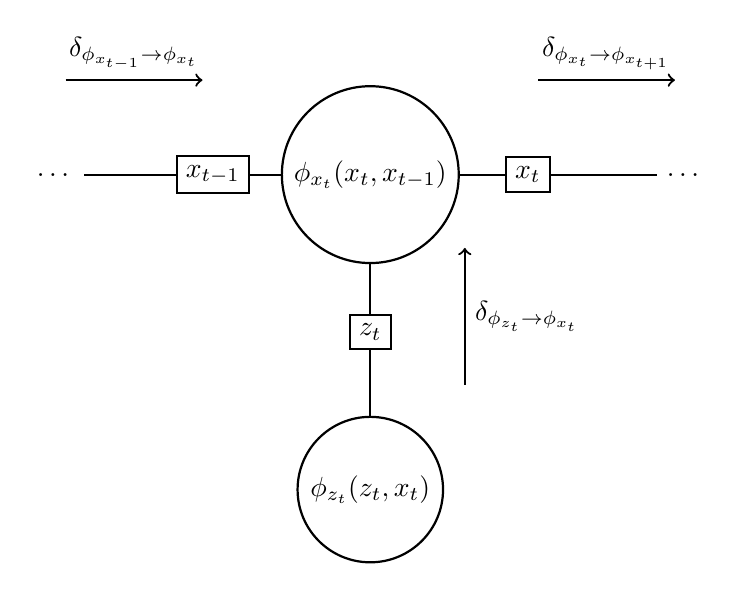
\begin{tikzpicture}[scale=0.80]
\begin{scope}[every node/.style={circle,thick,draw}]
    \node (xt) at (0, 0) {$\phi_{\pmb{x}_t} (\pmb{x}_{t}, \pmb{x}_{t-1})$};
    \node (zt) at (0, -5) {$\phi_{\pmb{z}_t} (\pmb{z}_{t}, \pmb{x}_{t})$};
\end{scope}

\begin{scope}[every node/.style={thick,draw}]
	\node (sx{t-1}) at (-2.5, 0) {$\pmb{x}_{t-1}$};
    \node (sxt) at (2.5, 0) {$\pmb{x}_{t}$};
    \node (szt) at (0, -2.5) {$\pmb{z}_{t}$};
\end{scope}

\begin{scope}[style={thick,draw}]
    \node (xdot0) at (-5,0) {\dots};
    \node (xdot1) at (5,0) {\dots};
    
    \node (a0t0) at (-5, 1.5) {};
    \node (a1t0) at (-2.5, 1.5) {};
    
    \node (a0t1) at (2.5, 1.5) {};
    \node (a1t1) at (5, 1.5) {};
    
    \node (a0z1) at (1.5, -3.5) {};
    \node (a1z1) at (1.5, -1) {};
    
\end{scope}

\begin{scope}[style={thick,draw}]	
	\path [-] (sx{t-1}) edge node {} (xt);
	\path [-] (xt) edge node {} (sxt);
	\path [-] (xt) edge node {} (szt);
	\path [-] (szt) edge node {} (zt);
	
	\path [-] (xdot0) edge node {} (sx{t-1});
	\path [-] (sxt) edge node {} (xdot1);
	
	\path [->, above] (a0t0) edge node {$\delta_{\phi_{\pmb{x}_{t-1}} \rightarrow \phi_{\pmb{x}_{t}}}$} (a1t0);
	\path [->, above] (a0t1) edge node {$\delta_{\phi_{\pmb{x}_{t}} \rightarrow \phi_{\pmb{x}_{t+1}}}$} (a1t1);
	\path [->, right] (a0z1) edge node {$\delta_{\phi_{\pmb{z}_{t}} \rightarrow \phi_{\pmb{x}_{t}}}$} (a1z1);
\end{scope}

\end{tikzpicture}

\caption[Message passing in a Kalman Filter.]{Message passing in a Kalman Filter.}
\label{figure:message_passing}
\end{figure}

\begin{align}
\delta_{\pmb{x}(t) \rightarrow \pmb{x}(t+1)}(\pmb{x}_{t}) &= \int \phi_{\pmb{x}(t)}(\pmb{x}_{t}, \pmb{x}_{t-1}) \delta_{\pmb{z}(t) \rightarrow \pmb{x}(t)} (\pmb{x}_{t})  \delta_{\pmb{x}(t-1) \rightarrow \pmb{x}(t)} (\pmb{x}_{t-1}) d\pmb{x}_{t-1} \nonumber \\
&= \underbrace{ \delta_{\pmb{z}(t) \rightarrow \pmb{x}(t)} (\pmb{x}_{t}) }_\text{\textit{Measurement update}} \underbrace{ \int \phi_{\pmb{x}(t)}(\pmb{x}_{t}, \pmb{x}_{t-1})  \delta_{\pmb{x}(t-1) \rightarrow \pmb{x}(t)} (\pmb{x}_{t-1}) d\pmb{x}_{t-1} }_\text{\textit{Prediction}} \label{eqn:state}
\end{align}

\begin{remark}
The notation in Equation~\ref{eqn:state} is unwieldy, but I couldn't think of anything else that wasn't ambiguous.
\end{remark}

\section{Part 1: Prediction}
\label{section:prediction}
Basically, evaluating this equation:

\begin{align}
\Psi(\pmb{x}_{t}) &= \int \phi_{\pmb{x}(t)}(\pmb{x}_{t}, \pmb{x}_{t-1})  \delta_{\pmb{x}(t-1) \rightarrow \pmb{x}(t)} (\pmb{x}_{t-1}) d\pmb{x}_{t-1}  \label{eqn:rec_bel}
\end{align}

\subsection{Canonical Form Representation}
\label{subsection:canonical}
Canonical form representation is consistent with~\cite{Koller_canonical}.

\subsubsection{The Initial Belief, $\phi_{\pmb{x}(t)} (\pmb{x}_{t}, \pmb{x}_{t-1})$}
\label{subsubsection:initial_pot}

The potential, $\phi_{\pmb{x}(t)} (\pmb{x}_{t}, \pmb{x}_{t-1})$, is the CPD:
\begin{align}
& \phi_{\pmb{x}(t)} (\pmb{x}_{t}, \pmb{x}_{t-1}) = \mathcal{N}\left(\pmb{x}_{t} | A_{t} \pmb{x}_{t-1} + B_{t} \pmb{x}_{t-1}, R_{t} \right) \nonumber \\
 &= \frac{1}{ (2 \pi)^{n/2}| R_{t} |^{1/2} } \exp{ \{ -\frac{1}{2} \left( \pmb{x}_{t} - A_{t} \pmb{x}_{t-1} - B_{t} \pmb{x}_{t-1} \right)^{T} R_{t}^{-1} \left( \pmb{x}_{t} - A_{t} \pmb{x}_{t-1} - B_{t} \pmb{x}_{t-1} \right)\} }
\end{align}
It can be rearranged as a joint density function as follows:
\begin{align}
& -\frac{1}{2} \left( \pmb{x}_{t} - A_{t} \pmb{x}_{t-1} - B_{t} \pmb{x}_{t-1} \right)^{T} R_{t}^{-1} \left( \pmb{x}_{t} - A_{t} \pmb{x}_{t-1} - B_{t} \pmb{x}_{t-1} \right) \nonumber \\
&= -\frac{1}{2} \begin{bmatrix} \left( \pmb{x}_{t} - B_{t} \pmb{u}_{t} \right)^{T} & \pmb{x}_{t-1}^{T} \end{bmatrix} \begin{bmatrix} R_{t}^{-1} & -R_{t}^{-1} A_{t} \\ -A_{t}^{T} R_{t}^{-1} & A_{t}^{T} R_{t}^{-1} A_{t} \end{bmatrix} \begin{bmatrix} \left( \pmb{x}_{t} - B_{t} \pmb{u}_{t} \right) \\ \pmb{x}_{t-1} \end{bmatrix} \nonumber \\
&= -\frac{1}{2} \left( \pmb{X}_{t} - \pmb{M}_t \right)^{T} P_t \left( \pmb{X}_{t} - \pmb{M}_t \right) 
\end{align}
Where,
\begin{align}
\pmb{X}_{t} &= \begin{bmatrix} \pmb{x}_t \\ \pmb{x}_{t-1} \end{bmatrix} \\
\pmb{M}_t &= \begin{bmatrix} B_{t}\pmb{u}_t \\ \pmb{0} \end{bmatrix} \\
P_t &= \begin{bmatrix} R_{t}^{-1} & -R_{t}^{-1} A_{t} \\ -A_{t}^{T} R_{t}^{-1} & A_{t}^{T} R_{t}^{-1} A_{t} \end{bmatrix}
\end{align}
The joint density can now be easily represented in canonical form:
\begin{align}
\phi_{\pmb{x}(t)} (\pmb{x}_{t}, \pmb{x}_{t-1}) &= \mathcal{N}\left( \pmb{X} | \pmb{M}, P \right) \nonumber \\
&= \mathcal{C} \left( \pmb{x}_t, \pmb{x}_{t-1} ; P_t, \pmb{h}_{t}, g_{t} \right)
\end{align}
Where, 
\begin{align}
\pmb{h}_{t} &= P_{t} \pmb{M}_{t} \\
g_{t} &= -\frac{1}{2} \pmb{M}^{T}_{t} P_{t} \pmb{M}_{t} - \ln{ \left\{ (2 \pi)^{n/2} | R_{t} |^{1/2} \right\} }
\end{align}
\begin{remark}
I introduced $\pmb{X}_{t}$ just to show the new arrangement was in quadratic form, I find it easier to show full scope in canonical form  so I don't lose track of anything.
\end{remark}

\subsubsection{The Recursive Belief, $\delta_{\pmb{x}(t-1) \rightarrow \pmb{x}(t)} (\pmb{x}_{t-1})$}
\label{subsubsection:rec_bel}

$\delta_{\pmb{x}(t-1) \rightarrow \pmb{x}(t)} (\pmb{x}_{t-1})$ is some unknown distribution which can be represented generally in canonical form:
\begin{align}
\delta_{\pmb{x}(t-1) \rightarrow \pmb{x}(t)} (\pmb{x}_{t-1})&= \mathcal{C}\left( \pmb{x}_{t-1}; P_{t-1}, \pmb{h}_{t}, g_{t-1} \right) 
\end{align}
Where, 
\begin{align}
P_{t-1} &= \Sigma^{-1}_{t-1} \\
\mathbf{h}_{t-1} &= \Sigma_{t-1}^{-1} \pmb{\mu}_{t-1} \\
g_{t-1} &= -\frac{1}{2}\pmb{\mu}^{T} \Sigma_{t-1}^{-1} \pmb{\mu} - \ln{ \left\{ (2 \pi)^{n/2} | \Sigma_{t-1} |^{1/2} \right\} }
\end{align}
Since $  \delta_{\pmb{x}(t-1) \rightarrow \pmb{x}(t)} (\pmb{x}_{t-1}) $'s scope is a subset of $\phi_{\pmb{x}(t)} (\pmb{x}_{t}, \pmb{x}_{t-1})$'s, its variables must be augmented with zeros:
\begin{align}
P'_{t-1} &= \begin{bmatrix} 0 & -0 \\ 0 &  \Sigma^{-1}_{t-1} \end{bmatrix}\\
\mathbf{h}'_{t-1} &= \begin{bmatrix} \pmb{0} \\ \Sigma_{t-1}^{-1} \pmb{\mu}_{t-1} \end{bmatrix} 
\end{align}

 
\subsection{Belief Update}
\label{section:belief_update}

\begin{align}
\phi_{\pmb{x}(t)}(\pmb{x}_{t}, \pmb{x}_{t-1}) \delta_{\pmb{x}(t-1) \rightarrow \pmb{x}(t)} (\pmb{x}_{t-1}) &= 
\mathcal{C} \left( \pmb{x}_t, \pmb{x}_{t-1} ; P_t, \pmb{h}_{t}, g_{t} \right) \cdot \mathcal{C} \left( \pmb{x}_{t-1}; P'_{t-1}, \pmb{h}'_{t}, g_{t-1} \right) \nonumber \\
&= \mathcal{C} \left( \pmb{x}_t, \pmb{x}_{t-1}; P_{t} + P'_{t-1}, \pmb{h}_{t} + \pmb{h}'_{t-1}, g_{t} + g_{t-1} \right) \nonumber \\
&= \mathcal{C} \left( \pmb{x}_t, \pmb{x}_{t-1}; \hat{P}_{t}, \hat{\pmb{h}}_{t}, \hat{g}_{t} \right) 
\end{align}
\begin{align}
\hat{P}_{t} &= P_{t} + P'_{t-1} \nonumber  \\ 
&=  \begin{bmatrix} R_{t}^{-1} & -R_{t}^{-1} A_{t} \\ -A_{t}^{T} R_{t}^{-1} & A_{t}^{T} R_{t}^{-1} A_{t} \end{bmatrix} +  \begin{bmatrix} 0 & -0 \\ 0 &  \Sigma^{-1}_{t-1} \end{bmatrix} \nonumber \\
&= \begin{bmatrix} R_{t}^{-1} & -R_{t}^{-1} A_{t} \\ -A_{t}^{T} R_{t}^{-1} & A_{t}^{T} R_{t}^{-1} A_{t} +  \Sigma^{-1}_{t-1} \end{bmatrix} \\
\hat{\pmb{h}}_{t} &= \pmb{h}_t + \pmb{h}'_{t-1} \nonumber \\
&= \begin{bmatrix} R_{t}^{-1} B_{t} \pmb{u}_{t} \\ - A_{t}^{T} R_{t}^{-1} B_{t} \pmb{u}_{t}  \end{bmatrix} + \begin{bmatrix} \pmb{0} \\ \Sigma_{t-1}^{-1} \pmb{\mu}_{t-1} \end{bmatrix} \nonumber \\
&= \begin{bmatrix} R_{t}^{-1} B_{t} \pmb{u}_{t} \\ - A_{t}^{T} R_{t}^{-1} B_{t} \pmb{u}_{t} + \Sigma_{t-1}^{-1} \pmb{\mu}_{t-1} \end{bmatrix} \\
\hat{g}_{t} &= g_{t} + g_{t-1} \nonumber \\
&=  -\frac{1}{2}\pmb{M}_{t}^{T} P \pmb{M}_{t} - \ln{ \left\{  (2 \pi)^{n/2} |R_{t} |^{1/2} \right\} } + \pmb{\mu}^{T} \Sigma_{t-1}^{-1} \pmb{\mu} -\ln{ \left\{ (2 \pi)^{n/2} | \Sigma_{t-1} |^{1/2} \right\} }
\end{align}

\subsubsection{Marginalisation}
\label{subsubsection:marginalisation}
Evaluating Equation~\ref{eqn:state} according to~\cite{Koller_canonical}:
\begin{align}
\widetilde{P}_{t} &= R_{t}^{-1} - \left( A_{t}^{T} R_{t}^{-1} \right)^{T} \left( A_{t}^{T} R_{t}^{-1} A_{t} + \Sigma_{t-1}^{-1} \right)^{-1} \left( A_{t}^{T} R_{t}^{-1} \right) \label{eqn:p_direct} \\
\widetilde{\pmb{h}}_{t} &= R_{t}^{-1} B_{t} \pmb{u}_{t} + R_{t}^{-1}A_{t} \left(A_{t}^{T} R_{t}^{-1} A_{t} + \Sigma^{-1}_{t-1} \right)^{-1} \left( -A_{t}^{T} R_{t}^{-1} B_{t} \pmb{u}_{t} + \Sigma^{-1}_{t-1} \pmb{\mu}_{t-1} \right) \label{eqn:h_direct} \\
\widetilde{g}_{t} &= \hat{g}_{t} -\frac{1}{2} \left( -A_{t}^{T} R_{t}^{-1} B_{t} \pmb{u}_{t} + \Sigma^{-1}_{t-1} \pmb{\mu}_{t-1} \right)^{T} \left(A_{t}^{T} R_{t}^{-1} A_{t} + \Sigma^{-1}_{t-1} \right)^{-1} \left( -A_{t}^{T} R_{t}^{-1} B_{t} \pmb{u}_{t} + \Sigma^{-1}_{t-1} \pmb{\mu}_{t-1} \right) \nonumber
\end{align}
The current state belief, before the measurement update, is the following distribution:
\begin{align}
\Psi({\pmb{x}_{t}}) &= \mathcal{C}\left( \pmb{x}_{t}; \widetilde{P}_t, \widetilde{\pmb{h}}_{t}, \widetilde{g}_{t} \right)
\end{align}

\subsubsection{Simplifications}
\label{subsubsection:simplification}
The equations in Section~\ref{subsubsection:marginalisation} are horrific, but they can be reduced to something manageable by applying the Woodbury Matrix Identity (Lemma~\ref{theorem:woodbury}) to the following component:
\begin{align}
\left( A_{t}^{T} R_{t}^{-1} A_{t} + \Sigma^{-1}_{t-1} \right)^{-1} &= \left( \Sigma_{t-1} - \Sigma_{t-1} A_{t}^{T} \left( R_{t} + A_{t} \Sigma_{t-1} A_{t}^{T} \right)^{-1} A_{t} \Sigma_{t-1} \right) 
\end{align}
Then letting,
\begin{align}
\overline{\Sigma}_{t} &= R_{t} + A_{t} \Sigma_{t-1} A_{t}^{T}
\end{align}
\begin{remark}
If you don't follow the preceding steps, you will end with a perfectly valid set of equations but they won't be identical to the standard Kalman Filter Algorithm (defined in~\cite{Thrun_rec, Thrun_gauss}), which isn't as rewarding. 
\end{remark}
Simplifying Equation~\ref{eqn:p_direct}
\begin{align*}
\widetilde{P}_t &= R_{t}^{-1} - \left( A_{t}^{T} R_{t}^{-1} \right)^{T} \left( \Sigma_{t-1} - \Sigma_{t-1} A_{t}^{T} \left( R_{t} + A_{t} \Sigma_{t-1} A_{t}^{T} \right)^{-1} A_{t} \Sigma_{t-1} \right)  \left( A_{t}^{T} R_{t}^{-1} \right) \\
&= R_{t}^{-1} - \left( A_{t}^{T} R_{t}^{-1} \right)^{T} \left( \Sigma_{t-1} - \Sigma_{t-1} A_{t}^{T} \overline{\Sigma}_{t}^{-1} A_{t} \Sigma_{t-1} \right)  \left( A_{t}^{T} R_{t}^{-1} \right) \\
&= R_{t}^{-1} - R_{t}^{-1} \left(A_{t} \Sigma_{t-1} A_{t}^{T} \right) R_{t}^{-1} + R_{t}^{-1} \left(A_{t} \Sigma_{t-1} A_{t}^{T} \right) \overline{\Sigma_{t}^{-1}} \left(A_{t} \Sigma_{t-1} A_{t}^{T} \right) R_{t}^{-1} \\
&= R_{t}^{-1} - R_{t}^{-1} \left( \overline{\Sigma}_{t} - R_{t} \right) R_{t}^{-1} + R_{t}^{-1} \left( \overline{\Sigma}_{t} - R_{t} \right) \overline{\Sigma_{t}^{-1}} \left( \overline{\Sigma}_{t} - R_{t} \right) R_{t}^{-1} \\
&= R_{t}^{-1} - R_{t}^{-1} \overline{\Sigma}_{t} R_{t}^{-1} - R_{t}^{-1} - R_{t}^{-1} \left(I - R_{t} \overline{\Sigma}_{t}^{-1}  \right) \left( I - \left( R_{t} \overline{\Sigma}_{t} \right)^{-1} \right) \\
&=  2 R_{t}^{-1} -R_{t}^{-1} \overline{\Sigma}_{t} R_{t}^{-1} + R_{t}^{-1} \left( I - R_{t} \overline{\Sigma}^{-1}_{t} - \left( R_{t} \overline{\Sigma}_{t} \right)^{-1} + I \right) \\
&= 2 R_{t}^{-1} -R_{t}^{-1} \overline{\Sigma}_{t} R_{t}^{-1} -2 R_{t}^{-1} + \overline{\Sigma}^{-1}_{t} + R_{t}^{-1} \overline{\Sigma}_{t} R_{t}^{-1} \\
&= \overline{\Sigma}^{-1}_{t} \numberthis
\end{align*}
Simplifying Equation~\ref{eqn:h_direct}:
\begin{align*}
\widetilde{\pmb{h}}_{t} &= R_{t}^{-1} B_{t} \pmb{u}_{t} + R_{t}^{-1}A_{t} \left( \Sigma_{t-1} - \Sigma_{t-1} A_{t}^{T} \left( R_{t} + A_{t} \Sigma_{t-1} A_{t}^{T} \right)^{-1} A_{t} \Sigma_{t-1} \right)  \left( -A_{t}^{T} R_{t}^{-1} B_{t} \pmb{u}_{t} + \Sigma^{-1}_{t-1} \pmb{\mu}_{t-1} \right) \\
&= R_{t}^{-1} B_{t} \pmb{u}_{t} + R_{t}^{-1}A_{t} \left( \Sigma_{t-1} - \Sigma_{t-1} A_{t}^{T} \overline{\Sigma}_{t}^{-1}  A_{t} \Sigma_{t-1} \right)  \left( -A_{t}^{T} R_{t}^{-1} B_{t} \pmb{u}_{t} + \Sigma^{-1}_{t-1} \pmb{\mu}_{t-1} \right) \\
&= R_{t}^{-1} B_{t} \pmb{u}_{t}  - R_{t}^{-1} \left( A_{t} \Sigma_{t-1} A_{t}^{T} \right) R_{t}^{-1} B_{t} \pmb{u}_{t} + R_{t}^{-1} \left( A_{t} \Sigma_{t-1} A_{t}^{T} \right)  \overline{\Sigma}_{t}^{-1} \left( A_{t} \Sigma_{t-1} A_{t}^{T} \right)  R_{t}^{-1} B_{t} \pmb{u}_{t} \\
&\ + R_{t}^{-1} A_{t} \left( \Sigma_{t-1} \Sigma_{t-1}^{-1} \right) \pmb{\mu}_{t-1} - R_{t}^{-1} \left( A_{t} \Sigma_{t-1} A_{t}^{T} \right) \overline{\Sigma}^{-1}_{t} A_{t} \left( \Sigma_{t} \Sigma_{t}^{-1} \right) \pmb{\mu}_{t-1} \\
&= R_{t}^{-1} B_{t} \pmb{u}_{t}  - R_{t}^{-1} \left( \overline{\Sigma}_{t} - R_{t}  \right) R_{t}^{-1} B_{t} \pmb{u}_{t} + R_{t}^{-1} \left( \overline{\Sigma}_{t} - R_{t} \right)  \overline{\Sigma}_{t}^{-1} \left( \overline{\Sigma}_{t} - R_{t} \right)  R_{t}^{-1} B_{t} \pmb{u}_{t} \\
&\ + R_{t}^{-1} A_{t} \pmb{\mu}_{t-1} - R_{t}^{-1} \left( \overline{\Sigma}_{t} - R_{t} \right) \overline{\Sigma}^{-1}_{t} A_{t}  \pmb{\mu}_{t-1} \\
&= R_{t}^{-1} \left( A_{t} \pmb{\mu}_{t-1} + B_{t} \pmb{u}_{t} \right) - R_{t}^{-1} \left( \overline{\Sigma}_{t} - R_{t} \right) \left( I - \overline{\Sigma}^{-1}_{t} \left( \overline{\Sigma}_{t} - R_{t} \right) \right) R_{t}^{-1} B_{t} \pmb{u}_{t} - R_{t}^{-1} \left( \overline{\Sigma}_{t} - R_{t} \right) \overline{\Sigma}_{t}^{-1} A_{t} \pmb{\mu}_{t} \\
&= R_{t}^{-1} \left( A_{t} \pmb{\mu}_{t-1} + B_{t} \pmb{u}_{t} \right) - R_{t}^{-1} \left( \overline{\Sigma}_{t} - R_{t} \right) \overline{\Sigma}^{-1}_{t} \left( R_{t} R_{t}^{-1} \right) B_{t} \pmb{u}_{t} - R_{t}^{-1} \left( \overline{\Sigma}_{t} - R_{t} \right) \overline{\Sigma}_{t}^{-1} A_{t} \pmb{\mu}_{t} \\
&= R_{t}^{-1} \left( A_{t} \pmb{\mu}_{t-1} + B_{t} \pmb{u}_{t} \right) - R_{t}^{-1} \left( \overline{\Sigma}_{t} - R_{t} \right) \overline{\Sigma}_{t}^{-1} \left( A_{t} \pmb{\mu}_{t-1} - B_{t}\pmb{u}_{t} \right) \\
&= R_{t}^{-1} \left( I  - \left( \overline{\Sigma}_{t} - R_{t} \right) \overline{\Sigma}^{-1}_{t} \right) \left( A_{t} \pmb{\mu}_{t-1} + B_{t} \pmb{u}_{t} \right) \\
&= \left(  R_{t}^{-1} R_{t} \right) \overline{\Sigma}^{-1}_{t} \left( A_{t} \pmb{\mu}_{t-1} + B_{t} \pmb{u}_{t} \right) \\
&= \overline{\Sigma}^{-1}_{t} \left( A_{t} \pmb{\mu}_{t-1} + B_{t} \pmb{u}_{t} \right) \numberthis 
\end{align*}
From the definition of the information vector~\cite{Koller_canonical}:
\begin{align*}
\widetilde{\pmb{h}}_{t} &= \widetilde{P}_{t} \widetilde{\pmb{\mu}}_t \\
\therefore \widetilde{\pmb{\mu}}_{t} &= \widetilde{P}_{t}^{-1} \widetilde{\pmb{h}}_{t}  \\
&= \left( \overline{\Sigma}^{-1}_{t} \overline{\Sigma}_{t} \right) \left( A_{t} \pmb{\mu}_{t-1} + B_{t} \pmb{u}_{t} \right) \\
&= A_{t} \pmb{\mu}_{t-1} + B_{t} \pmb{u}_{t}  \numberthis
\end{align*}

\newpage
\begin{theo}[Specialised Woodbury Inversion Identity\footnote{This is directly stolen, with a few added steps, from~\cite{Thrun_gauss}. This is also referred to as the Sherman-Morrison-Woodbury Inversion Identity.}] \label{theorem:woodbury}
For any invertible quadratic matrices $R$ and $Q$ and any matrix $P$ with appropriate dimensions, the following holds true
\begin{align*}
(R + P Q P^{T} )^{-1} &= R^{-1} - R^{-1} P (Q^{-1} + P^{T} R^{-1} P)^{-1} P^{T} R^{-1}
\end{align*}
\noindent \textbf{Proof}: Define $\Psi = (Q^{-1} + P^{T} R^{-1} P )^{-1}$. It suffices to show that
\begin{align*}
(R^{-1} - R^{-1} P \Psi P^{T} R^{-1})(R + P Q P) &= I 
\end{align*}
This is shown through a series of transformations
\begin{align*}
&= R^{-1} R - R^{-1} P Q P^{T} - R^{-1} P \Psi P^{T} R^{-1} R + R^{-1} P \Psi P^{T} R^{-1} P Q P^{T}  \\ 
&= I + R^{-1} P Q P^{T} - R^{-1} P \Psi P^{T} - R^{-1} P \Psi P^{T} R^{-1} P Q P^{T}  \\
&= I + R^{-1} P \left[ Q P^{T} - \Psi P^{T} - \Psi P^{T} R^{-1} P Q P^{T} \right]  \\
&= I + R^{-1} P \left[ Q P^{T} - \Psi Q^{-1} Q P^{T} - \Psi P^{T} R^{-1} P Q P^{T} \right]  \\
&= I + R^{-1} P \left[ Q P^{T} - \Psi \left[ Q^{-1} + P^{T} R^{-1} P \right] Q P^{T} \right]  \\
&= I + R^{-1} P \left[ Q P^{T} - \Psi \Psi^{-1} Q P^{T} \right] \\
&= I + R^{-1} P \left[ I - I \right] Q P^{T}  \\
&= I \nonumber
\end{align*}
\end{theo}

\section{Part 2: Measurement Update}
\label{section:prediction}
The state estimate is finally completed by incorporating the current measurement, $\pmb{z}_{E, t}$.
\begin{align}
\delta_{\pmb{z}(t) \rightarrow \pmb{x}(t)} (\pmb{x}_{t}) &= \delta_{\phi_{\pmb{z}_{t}} \rightarrow \phi_{\pmb{x}_{t}}} (\pmb{x}_{t}) \cdot \Psi (\pmb{x}_{t}) 
\end{align}

\subsection{Canonical From Representation}
\label{subsection:measurement_canonical}
Once again a CPD is rearranged into a joint density:
\begin{align*}
\phi_{ \pmb{z}_{t} } ( \pmb{x}_{t}, \pmb{z}_{t} )&= \mathcal{N} \left( \pmb{z}_{t} | C_{t} \pmb{x}_{t}, Q_{t} \right) \\
&= \frac{1}{(2 \pi)^{k/2}| Q_{t} |^{(1/2)} } \exp{\left\{ -\frac{1}{2} \left(  \pmb{z}_{t} - C_{t}\pmb{x}_{t} \right)^{T} Q_{t}^{-1} \left(  \pmb{z}_{t} - C_{t}\pmb{x}_{t} \right) \right\} } \numberthis
\end{align*}
\begin{align*}
& -\frac{1}{2} \left(  \pmb{z}_{t} - C_{t}\pmb{x}_{t} \right)^{T} Q_{t}^{-1} \left(  \pmb{z}_{t} - C_{t}\pmb{x}_{t} \right) \\
&= \begin{bmatrix} \pmb{x}^{T}_{t} & \pmb{z}^{T}_{t} \end{bmatrix} \begin{bmatrix} C_{t}^{T} Q_{t}^{-1} C_{t} & -C_{t}^{T} Q_{t}^{-1} \\  -Q_{t}^{-1} C_{t}^{T} & Q_{t}^{-1} \end{bmatrix}
\begin{bmatrix} \pmb{x}_{t} \\ \pmb{z}_{t} \end{bmatrix} \\
&= \left( \pmb{Z}_{t} \right)^{T} P_{\pmb{z}_{t}} \left( \pmb{Z}_{t} \right)
\end{align*}
Where,
\begin{align}
\pmb{Z}_{t} &= \begin{bmatrix} \pmb{x}_{t} \\ \pmb{z}_{t} \end{bmatrix} \\
P_{\pmb{z}_{t}} &= \begin{bmatrix} C_{t}^{T} Q_{t}^{-1} C_{t} & -C_{t}^{T} Q_{t}^{-1} \\  -Q_{t}^{-1} C_{t}^{T} & Q_{t}^{-1} \end{bmatrix} 
\end{align}
Resulting in the zero mean distribution,
\begin{align}
\phi_{ \pmb{z}_{t} } ( \pmb{x}_{t}, \pmb{z}_{t} )&= \mathcal{C} \left( \pmb{x}_{t}, \pmb{z}_{t} ; P_{\pmb{z}_t}, \pmb{0} , g_{\pmb{z}_t} \right) 
\end{align}
Where,
\begin{align}
g_{\pmb{z}_{t}} &= - \ln{ \left\{ (2 \pi)^{k/2} | Q_{t} |^{1/2} \right\} }
\end{align}

\subsubsection{Observations}
\label{subsubsection:observations}
The measurement of the current state is made, $\pmb{z}_{t} = \pmb{z}_{E, t}$. According to~\cite{Koller_canonical}:
\begin{align}
\widetilde{P}_{\pmb{z}_{t}} &= C_{t}^{T} Q_{t}^{-1} C_{t} \\
\widetilde{\pmb{h}}_{\pmb{z}_{t}} &= C_{t}^{T} Q_{t}^{-1}  \pmb{z}_{E, t} \\
\widetilde{g}_{\pmb{z}_{t}} &= - \ln{ \left\{ (2 \pi)^{k/2} | Q_{t} |^{1/2} \right\} } - \frac{1}{2} \pmb{z}_{t}^{T} Q_{t}^{-1} \pmb{z}_{t}
\end{align}
Therefore,
\begin{align}
\delta_{\pmb{z}(t) \rightarrow \pmb{x}(t)} (\pmb{x}_{t}) &= \phi_{ \pmb{z}(t) } ( \pmb{x}_{t} ) = \mathcal{C} \left( \pmb{x}_{t}; \overline{P}_{\pmb{z}_{t}}, \overline{\pmb{h}}_{\pmb{z}_{t}} , \overline{g}_{\pmb{z}_{t}}  \right) 
\end{align}

\subsection{Update and Simplifications}
\label{subsection:actual_update}
Finally, the measurement update is performed:
\begin{align*}
\delta_{\phi_{\pmb{x}_{t}} \rightarrow \phi_{\pmb{x}_{t+1}}}(\pmb{x}_{t}) &= \delta_{\phi_{\pmb{z}_{t}} \rightarrow \phi_{\pmb{x}_{t}}} (\pmb{x}_{t}) \cdot \Psi (\pmb{x}_{t}) \\
&= \mathcal{C}\left( \pmb{x}_{t}; \widetilde{P}_{\pmb{z}_{t}}, \widetilde{\pmb{h}}_{\pmb{z}_{t}} , \widetilde{g}_{\pmb{z}_{t}}  \right) \cdot \mathcal{C}\left( \pmb{X}_{t}; \widetilde{P}_t, \widetilde{\pmb{h}}_{t}, \widetilde{g}_{t} \right) \\
&= \mathcal{C}\left( \pmb{x}_{t}; \widetilde{P}_t + \widetilde{P}_{\pmb{z}_{t}}, \widetilde{\pmb{h}}_{t} + \widetilde{\pmb{h}}_{\pmb{z}_{t}}, \widetilde{g}_{t} + \widetilde{g}_{\pmb{z}_{t}} \right) \\
&= \mathcal{C}\left( \pmb{x}_{t}; \overline{P}_t, \overline{\pmb{h}}_{t}, \overline{g}_{t} \right) \numberthis
\end{align*}
Where,
\begin{align}
\overline{P}_{t} &= \overline{\Sigma}^{-1}_{t} + C_{t}^{T} Q_{t}^{-1} C_{t} \\
\overline{\pmb{h}}_{t} &= C_{t}^{T} Q_{t}^{-1} \pmb{z}_{E, t} + \overline{\Sigma}^{-1}_{t} \overline{\pmb{\mu}}_{t}
\end{align}
The precision matrix, $\overline{P}_{t}$, is defined as the inverse of the covariance matrix, therefore:
\begin{align}
\Sigma_{t} &= \left(  \overline{\Sigma}^{-1}_{t} + C_{t}^{T} Q_{t}^{-1} C_{t} \right)^{-1}
\end{align}
Using Lemma~\ref{theorem:woodbury} again,
\begin{align}
\Sigma_{t} &= \left( \overline{\Sigma}_{t} - \overline{\Sigma}_{t}  C_{t}^{T} \left( Q_{t} + C_{t} \overline{\Sigma}_{t} C_{t}^{T} \right)^{-1} C_{t} \overline{\Sigma}_{t}  \right) 
\end{align}
Defining the Kalman Gain, $K_{t}$, as:
\begin{align}
K_{t} &= \overline{\Sigma}_{t}  C_{t}^{T} \left( Q_{t} + C_{t} \overline{\Sigma}_{t} C_{t}^{T} \right)^{-1} \\
\therefore \Sigma_{t} &= \left( I - K_{t} C_{t} \right) \overline{\Sigma}_{t}
\end{align}
From the definition of the information vector~\cite{Koller_canonical}:
\begin{align*}
& \overline{\pmb{h}}_{t} =  \Sigma^{-1}_{t} \pmb{\mu}_t \\
& \therefore \pmb{\mu}_{t} = \Sigma_{t} \overline{\pmb{h}}_{t}  \\
&= \left( I - K_{t} C_{t} \right) \overline{\Sigma}_{t} \left( C_{t}^{T} Q_{t}^{-1} \pmb{z}_{E, t} + \overline{\Sigma}^{-1}_{t} \widetilde{\pmb{\mu}}_{t} \right) \\
&= \left( I - K_{t} C_{t} \right) \overline{\Sigma}_{t} C_{t}^{T} Q_{t}^{-1} \pmb{z}_{E, t} + \left( I - K_{t} C_{t} \right) \left( \overline{\Sigma}_{t} \overline{\Sigma}^{-1}_{t} \right) \widetilde{\pmb{\mu}}_{t} \\
&=  \left( \overline{\Sigma}_{t} C_{t}^{T} - K_{t} C_{t} \overline{\Sigma}_{t} C_{t}^{T} \right) Q_{t}^{-1} \pmb{z}_{E, t} + \left( I - K_{t} C_{t} \right) \widetilde{\pmb{\mu}}_{t} \numberthis
\end{align*}
A quick sidestep,
\begin{align*}
& K_{t} = \overline{\Sigma}_{t}  C_{t}^{T} \left( Q_{t} + C_{t} \overline{\Sigma}_{t} C_{t}^{T} \right)^{-1} \\
& K_{t}  \left( Q_{t} + C_{t} \overline{\Sigma}_{t} C_{t}^{T} \right) = \overline{\Sigma}_{t}  C_{t}^{T} \\
& K_{t} Q_{t} = \overline{\Sigma}_{t} C_{t}^{T} - K_{t} C_{t} \overline{\Sigma}_{t} C_{t}^{T}  \numberthis
\end{align*}
Now,
\begin{align*}
\pmb{\mu}_{t} &= \left( K_{t} Q_{t} \right) Q_{t}^{-1} \pmb{z}_{E, t} + \left( I - K_{t} C_{t} \right)  \widetilde{\pmb{\mu}}_{t} \\
&= K_{t} \left( Q_{t} Q_{t}^{-1} \right) \pmb{z}_{E, t} + \overline{\pmb{\mu}}_{t} - K_{t} C_{t} \widetilde{\pmb{\mu}}_{t} \\
&= \widetilde{\pmb{\mu}_{t}} + K_{t} \left( \widetilde{\pmb{\mu}}_{t} - C_{t} \pmb{z}_{E, t} \right) \numberthis
\end{align*}
\begin{remark}
You may notice I have neglected the scalar $\overline{g}_{t}$, it didn't really contain any of the really interesting equations. I assume it evaluates to a valid normalization constant as we have operated in a linear Gaussian system.
\end{remark}